\documentclass[12pt,preprint]{aastex}

\usepackage{latexsym}
\usepackage{fancybox}
\usepackage{graphicx}
\usepackage{amssymb}
\usepackage{color}
\usepackage{ulem}
\usepackage{float}
\usepackage{multicol}
\usepackage{enumitem}
\usepackage[hidelinks]{hyperref}
%\usepackage{setspace}
\usepackage{xcolor}  % for the links
\hypersetup{
    colorlinks,
    linkcolor={red!50!black},
    citecolor={blue!50!black},
    urlcolor={blue!80!black}
}

\pretolerance=10000
\textwidth=6.5in
\textheight=9.2in
\voffset = 0.0in
\topmargin=0.0in
\headheight=0.00in
\hoffset = 0.0in
\headsep=0.20in
\oddsidemargin=0in
\evensidemargin=0in
\parindent=2em
\parskip=0.25ex
 
%\input{defs_xavier}
%\input{/u/xavier/bin/latex}
%\input{/u/xavier/bin/defs}

\newcommand{\npair}{50}
\def\ssp{\def\baselinestretch{1.0}\large\normalsize}
\newcommand{\oneskip}{\vskip \baselineskip}
\newcommand{\annrev}{ARA\&A}
\newcommand{\za}{z$_{ abs}$}
\newcommand{\zg}{z$_{ galaxy}$}
\newcommand{\zl}{$z_{emitter}$}
\newcommand{\zf}{z$_{df}$}
\newcommand{\avxi}{$\langle\xi\rangle$}
\newcommand{\omg}{$\Omega_{g}(z)$}
\newcommand{\tu}{$\tau( > M)$}
\newcommand{\mc}{$10^{12}M_{\odot}$}
\def \lnhi {$\log N_{HI}$}
\def \cmm  {cm$^{-2}$}
\def \cmmm {cm$^{-3}$}
\def \hfreq {$f_{\rm{HI}} (N,X)$}
\def \gamrate {$\Gamma_{912}$}
\def \fn {$f_{\rm{HI}} (N,X)$}
\def \lyaf {Ly--$\alpha$ forest}
\def \nqso  {seven}
\def \cmm  {\rm cm^{-2}}
\newcommand{\lya}{Ly$\alpha$}

\usepackage{multicol}

\newenvironment{my_itemize}{
\begin{itemize}
  \setlength{\itemsep}{1pt}
  \setlength{\parskip}{0pt}
  \setlength{\parsep}{0pt}}{\end{itemize}
}

\newenvironment{my_enumerate}{
\begin{enumerate}
  \setlength{\itemsep}{1pt}
  \setlength{\parskip}{0pt}
  \setlength{\parsep}{0pt}}{\end{enumerate}
}



\usepackage{geometry}
\geometry{letterpaper,tmargin=1.3in,bmargin=0.7in,lmargin=0.95in,rmargin=0.95in}
\usepackage[layout=modern]{advancedcoverpage}


\title{{\Large PYPIT:  A Data Reduction Pipeline for UCO and WMKO}}

\presentedto{{\large \underline{2017 UCO Call for mini-grants}} \\
\vskip 0.1in
{\it Submitted to the UCOAC}
}


\author{
{\bf PI:} 
J. Xavier Prochaska (UCSC) \\
\vskip 0.1in
{\bf UC Faculty/Staff/PhD Co-I's:} \\
William Deich (UCO) \\
Joseph F. Hennawi (UCSB) \\
Tiffany Hsyu (UCSC) \\
Carl Melis (UCSD) \\
\vskip 0.1in
\vskip 0.1in
{\bf other Co-I's:} \\
R. Cooke (Durham), Luca Rizzi (WMKO) \\
\vskip 0.3in
%\includegraphics[width=5.5in]{../WhitePaper/title_fig2.pdf}
{\bf Abstract:} \\
We request a UCO mini-grant to fund the development of PYPIT,
an open source python based data reduction pipeline for echelle, longslit, and multi-slit
observations on UCO optical and near-IR spectrometers.
This project is being pursued in collaboration with WMKO,
following the recommendation of the Keck SSC.
To meet UCO's commitment and expand the capability
to other Lick Observatory instruments, we require the
funding requested within.
}

 
\begin{document}
\maketitle

	\pagestyle{myheadings}    % Go for customized headings
%\markright{Prochaska--U079 2008A Proposal---Quasars Probing Quasars}
	\markboth{\hfill Prochaska -- PYPIT (v1.1) \hfill}{\hfill
          Prochaska -- PYPIT (v1.1) \hfill}



%%%%%%%%%%%%%%%%%%%%%%%%%%%%%%%%%%%%%%%%%%%%%%%%%%%%%%%%%%%%%
%\vskip 0.2in

\noindent {\bf Introduction:} For the past several years, we have been developing a Python
based data reduction pipeline (DRP) named PYPIT\footnote{
\href{https://github.com/PYPIT/PYPIT}{PYPIT github repository};
\href{http://pypit.readthedocs.io/en/latest/}{PYPIT docs}}.
While driven initially and primarily by our own scientific
needs, we designed and built the PYPIT architecture
with several guiding philosophies that enable it to be used more generally:

\vskip -0.2in

\begin{my_itemize}
\item Python (2.7 and 3.6)
\item Implement modern practices for shared code development 
(i.e.\ git, github)
\item Encourage community usage and contributions
\item Include minimal dependencies (emphasis on numpy, scipy, astropy)
\item Construct unit tests and data
\href{https://github.com/PYPIT/PYPIT-development-suite}{test suites}
with 
\href{https://travis-ci.org/PYPIT/PYPIT/}{continuous integration}
\item Integrate with WMKO and the broader community (e.g.\ {\it astropy})
\end{my_itemize}

\vskip -0.1in

\noindent
In April 2017, we released v0.2 of PYPIT which included 
support for Keck/LRIS and Lick/Kast. 
%, and echelle spectrometers(APF, HIRES).
In Spring/Summer 2017, we were invited to participate
in the WMKO-led Data Reduction Working Group (DRWG). We 
\href{https://www.dropbox.com/s/n17il1aah1xs6fx/ucsc_pypit_mar2017.pdf?dl=0}
{presented} to that group our progress with PYPIT and
lessons learned from our 17+ years of DRP development in 
IDL.%\footnote{
%\href{http://www.ucolick.org/~xavier/LowRedux/}{LowRedux};
%\href{http://www.ucolick.org/~xavier/HIRedux/}{HIRedux}
%}.
We helped develop the recommendations of the DRWG as 
presented\footnote{\href{https://www.dropbox.com/s/k7ykp80voslaw7o/DRWG_June2017_SSC_v2.pptx?dl=0}{DRWG presentation}} 
to the Keck/SSC.  This presentation was well received by the
SSC, which recommended that we present a detailed development plan and a well defined set of requirements for DRP development.  As FY18 begins for WMKO,
we have agreed to spend Year~1 developing a DRP for WMKO
that supports all Longslit modes of Keck/LRIS (save polarimetry)
in a more modularized version of PYPIT, as well developing the
tools for full Multi-slit support. It is planned that this
will lay the foundation for all other future development of
spectroscopic DRPs at WMKO.
This proposal to the mini-grant process will fund
that activity at UCO (and more) while staff at WMKO
focus on updating the observing infrastructure to produce complete metadata (slitmask design software, instrument configuration manager and observations execution tools).%\footnote{WMKO requested additional
%resources for DRP development at IPAC in the NASA overguide.
%That proposal was well received but not funded.  We expect they
%will reapply in 2018.}


%%%%%%%%%%%%%%%%%%%%%%%%%
%%%%%%%%%%%%%%%%%%%%%%%%%
%\vskip 0.1in

\noindent 
{\bf Nuts and Bolts:} 
The requested funding from this mini-grant will support
several developments in PYPIT that will benefit the UC
community.  We describe each in turn and summarize the
timeline in Table~\ref{tab:timeline} and Figure~\ref{fig:PYPIT}.
We further emphasize that PYPIT is not a stand-alone,
one-year project;
the UCOAC should be prepared to receive future funding 
requests for the continued support of this software.


%%%%%%%%%%%%%%%%%%%%%%%%%
%\vskip -0.15in

\noindent 
{\it Core Development:} 
There are three core activities for PYPIT that demand the
skill set and focused dedication of a staff programmer
in UCO's Scientific Programming Group (SPG):

\vskip -0.15in

\begin{my_enumerate}

\vskip -0.15in

\item Refactor significant portions of the code to improve
modularity.  While PYPIT is built with standard classes 
and methods, it is not sufficiently modular.  This currently
inhibits efficient and effective development by the
community (or anyone new to the project).  This refactoring,
managed by lead developers Prochaska \& Cooke, 
will require two work months to complete by SPG staff.

\item Port all existing Cython code to Python.
For performance considerations, a number of low-level
routines of PYPIT were written in Cython.  We have
found these difficult to maintain and debug and have 
decided (following the DRWG recommendation) to port these
to Python.  We will also write complementary
unit tests [1.5 months work]. 

\item Initiate parallelization.  The obvious drawback
of coding in Python is performance and PYPIT suffers accordingly.
There are, however, several tasks which may be parallelized
for standard multi-core platforms using {\tt map/pool} methods.
We estimate 1.5~months of SPG effort to begin this work, 
focusing on the areas which would provide greatest 
improvement in computational time (e.g.\ sky subtraction). 
%(in particular, the routines for object/sky 
%boundary definition, sky subtraction, optimal extraction).
\end{my_enumerate}

\vskip -0.15in

\noindent
All three activities demand a professional programmer
and we request 0.5~FTE of SPG support at UCO where
the staff member can interact directly with PI Prochaska.

%%%%%%%%%%%%%%%%%%%%%%%%%
%\vskip -0.05in

\noindent 
{\it LRIS longslit:} 
The primary functional goal of Year~1 of the WMKO
DRP plan is to build a DRP that reduces any set 
of data with Keck/LRIS in both Longslit and Multi-Slit mode.
Currently, PYPIT supports several modes only in Longslit
(e.g.\ Figure~\ref{fig:LRIS_example}).
In 2018, we will incorporate all LRIS setups
and further integrate PYPIT into WMKO. The latter
involves 
(i) building a set of requirements for the DRP 
including metrics of data quality;
(ii) obtaining a test suite of LRIS spectra;
(iii) developing PYPIT accordingly.
This activity will be led by PI Prochaska
and we estimate 3~months of his effort; this
motivates the teaching buyout in 
Fall~2018.  As this development progresses,
we will begin a similar effort with DEIMOS, led
by Co-I Hennawi with advisement 
from M. Cooper (UCI).

%%%%%%%%%%%%%%%%%%%%%%%%%
\vskip 0.05in

\noindent 
{\it NIRSPEC low-dispersion:} 
Presently, PYPIT does not support any near-IR spectrograph.
While many of the core algorithms will seamlessly apply to 
such data, there are additional aspects of the near-IR that
need development, e.g.\  dark frames, ABBA image subtraction,
telluric fluxing.  We will expand PYPIT to include longslit
modes of NIRSPEC.  This effort will be led by PhD student
T. Hsyu who has previously contributed to PYPIT
(fluxing, coaddition, LRIS/Kast development).
We request 3~quarters of GSR support for her to 
complete this effort in 2018.  PI Prochaska will co-develop
and closely manage this portion of the project.


%%%%%%%%%%%%%%%%%%%%%%%%%
\vskip 0.05in


\noindent 
{\it HIRES:} 
Co-I Hennawi, who co-developed and maintains 
IDL-based DRPs for WMKO and UCO, will develop PYPIT 
for echelle observations with Keck/HIRES.
This builds upon Prof.\ Hennawi's previous efforts
with the IDL ESI pipeline. The groundwork for reducing
multi-order echelle data exist in beta versions of PYPIT, but
wavelength solutions and tools for combining orders are not 
yet implemented. 
We request one quarter of teaching buyout for 
him to complete this work and work on DEIMOS (above). 

%\noindent 
%{\it DEIMOS longslit:} 
%Co-I Hennawi will adapt PYPIT to reduce
%longslit observations with Keck/DEIMOS. This requires adding code to deal with the distinct
%DEIMOS detector layout and obtain wavelength solutions, which will pave the way for a future full DEIMOS
%Multi-slit pipeline. Prof.\ Hennawi
%has successfully performed preliminary PYPIT
%reductions on spectra with the 830G grating and in 2018 will 
%(i) complete and document this PYPIT development;
%(ii) expand the effort to include all other gratings.

%%%%%%%%%%%%%%%%%%%%%%%%%
\vskip 0.05in

\noindent 
{\it Hamilton echelle:}   In $\approx 11$~years of archived
Lick data, there are 1514 nights when the
Hamilton echelle was scheduled (3m and CAT nights). 
The Hamilton has not been used
on the 3m in nearly 10 months and with the advent of the APF is
essentially retired. Many of the Hamilton spectra
were taken to perform RV measurements
in the search of exoplanets.  Very few of these
(reduced) spectra, however, are in the public domain.
Co-I Melis will develop the echelle mode of PYPIT
to reduce the entire dataset.  He will then provide
the calibrated spectra in an easily accessible platform
for the UC community.  We budget 1~mo. of his effort.

%%%%%%%%%%%%%%%%%%%%%%%%%%
\clearpage

\begin{figure}
 \vskip -0.5in
\begin{center}
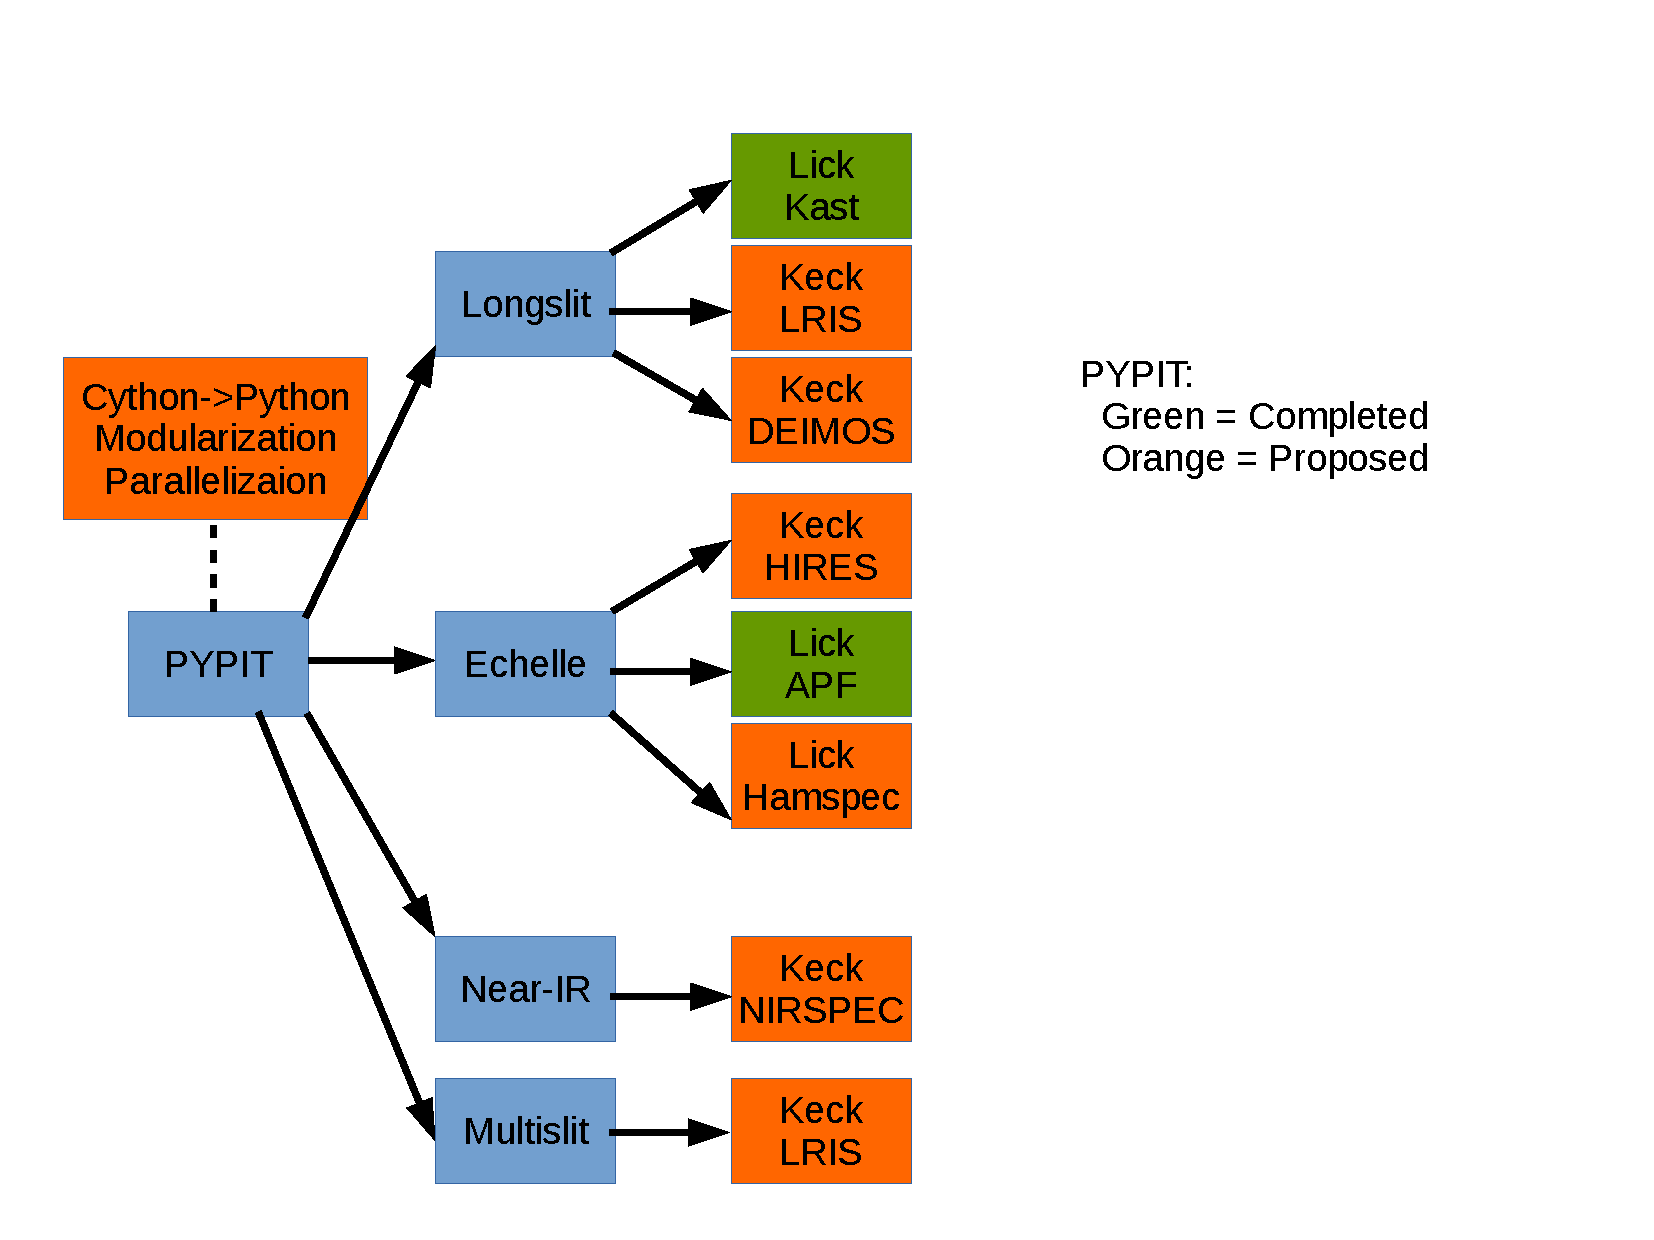
\includegraphics[scale=0.40]{code_sketch.pdf}
\end{center}
 \caption{\footnotesize  
Description of PYPIT as currently implemented (green)
and the proposed development (orange).
}\label{fig:PYPIT}
%  \end{minipage}
\end{figure}

\begin{figure}
 \vskip -0.5in
\begin{center}
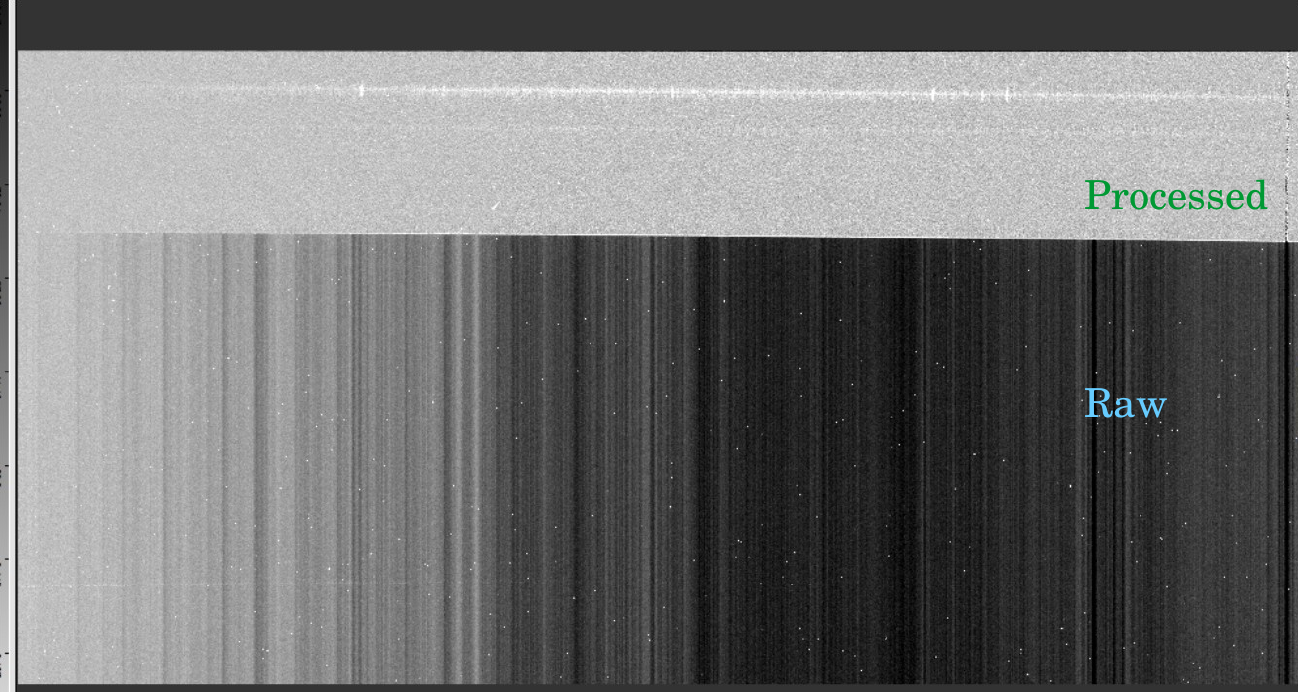
\includegraphics[scale=0.50]{processed_image.png}
\end{center}
 \caption{\footnotesize  
 Sky-subtracted image of an LRIS longslit exposure as 
 produced by the PYPIT software package.
}\label{fig:LRIS_example}
%  \end{minipage}
\end{figure}

\clearpage

{\footnotesize

\begin{table}[ht]
\begin{center}
\caption{Timeline \label{tab:timeline}}
\end{center}
\begin{tabular}{lcclccl}
\hline 
Activity & Begin & End & Description & Lead & Effort & Funding \\
\hline 
Modularize & 1/2018 & 12/2018 & Improve PYPIT modularity & SPG & 2 mo. & \$32,500 \\
%
Cython $\to$ Python & 1/2018 & 6/2018 & Convert Cython code to Python & SPG & 1.5 mo. & \$24,400 \\
%
Parallelization & 6/2018 & 12/2018 & Implement {\tt map/pool} methods & SPG & 1.5 mo. & \$24,400 \\
%%%%%%%
LRIS/Longslit & 1/2018 & 12/2018 & All modes (save polarimetry) & JXP & 4 mo. & 
\$12,000$^a$ \\
%%%%%%%
HIRES/Echelle & 1/2018 & 12/2018 & All grating & JFH & 3 mo. & \$12,000$^a$ \\
%%%%%%%
NIRSPEC & 1/2018 & 12/2018 & Low-dispersion modes & TH & 3 qrtrs & \$42,175$^b$\\
%%%%%%%
Hamilton & 3/2018 & 9/2018 & Reduce + archive & CM & 1 mo. & \$17,241 \\
\hline 
\end{tabular} 
${}^a$ Course relief \\
${}^b$ GSR\\
\end{table} 

}

\noindent
{\bf Salary, Benefits, Course Relief:} \\
The last column of Table 1 describes the costs
for each of the proposed activities.  These total
\$164,716.  While the UCOAC may be tempted to 
consider the above list a `menu', most of the items
are absolutely critical to the success of the
project.   We appreciate the total amount is substantial
but are also aware this is far less than any
serious other DRP effort on a first-class observatory
(e.g.\ {\it HST}, VLT).  \\

\noindent
{\bf Other funding requested:} \\
In addition to the funding covering work effort, we request
\$15,000 in funds to support the travel of Co-I's Hennawi, Melis,
Cooke and Rizzi to collaborate at UCO on PYPIT.  This will include
two hack-a-thons (we have held two in 2017).

\end{document}
